\chapter{Stato dell'arte}
\label{cha:statoArte}

\section{Reverse Proxy}
\begin{figure}[h!]
  \centering
  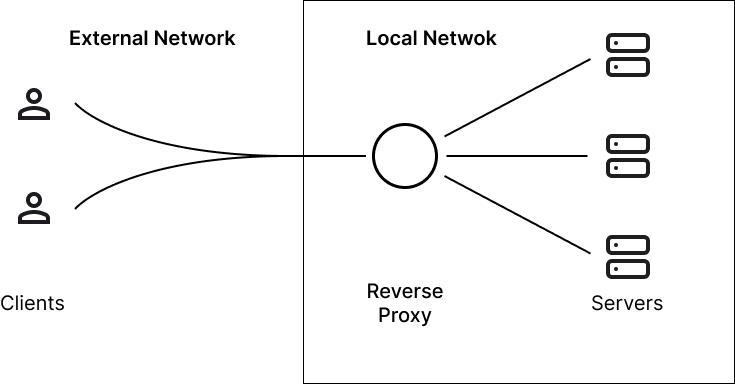
\includegraphics[width=.6\textwidth]{images/schema.png}
\end{figure}

\subsection{Cos'é}
Un reverse proxy è un dispositivo utilizzato nelle comunicazioni tra client e server. Questo dispositivo si interpone nelle comunicazioni nel lato dei server. Quindi viene utilizzato nella rete locale dove sono presenti i server e diventa l'unico nodo di accesso verso la rete globale. Ogni server quindi non sarà direttamente collegato al client che effettua la richiesta, ma é collegato al reverse proxy che successivamente inoltrerá le richieste ai relativi server e le risposte ai relativi client. Si fa ció cosí si diminuisce il carico di lavoro ai server perché non devono effettuare i controlli di sicurezza, che vengono invece effettuati direttamente dal reverse proxy. Inoltre, visto che tutte le comunicazioni passano per quel nodo, si può avere una visione piú generale di tutte le comunicazioni entranti e rilevare piú facilmente comportamenti anomali.
\subsubsection{Differenza con il forward proxy}
Il forward proxy è un dispositivo che funziona praticamente allo stesso modo peró si trova nella rete locale dei client. Quindi se si hanno più client ma si vuole avere solo un nodo di uscita verso la rete globale, si può utilizzare un forward proxy.

\subsection{Esempio comunicazione}
\subsubsection{Elementi}
Client: C\\ Reverse Proxy: R\\ Server1: S1; Server2: S2
\subsubsection{Configurazione Reverse Proxy}
\paragraph{Dominio} Come esempio consideriamo il dominio \textit{example.com}. Quindi il reverse proxy risponderá alle richieste fatte a \textit{*.example.com}.
\paragraph{Routing} Definiamo in base al subdomain quale server deve essere indirizzato
\begin{enumerate}
  \item primo.example.com - server1 (172.17.0.1)
  \item secondo.example.com - server2 (172.17.0.2)
\end{enumerate}
\subsubsection{Comunicazione}
\begin{enumerate}
  \item
  \begin{verbatim}
	GET /index.html HTTP/1.1
	Host: primo.example.com
  \end{verbatim}
	C manda una richiesta tramite il dominio \textit{primo.example.com}
  \item
	\begin{verbatim}
	GET /index.html HTTP/1.1
	Host: 172.17.0.1
	\end{verbatim}
	R riceve la richiesta, vede che il dominio indicato ha \textit{primo} come sottodominio. Controlla nella configurazione e vede che \textit{primo.example.com} é collegato a S1. Crea quindi una richiesta uguale a quella ricevuta, cambiando il destinatario e indicando l'indirizzo ip di S1.
  \item R riceve la risposta alla richiesta da S1.
  \item R invia la risposta ricevuta a C.
\end{enumerate}


\subsection{Perché viene utilizzato}
L'utilizzo di una struttura che si pone in mezzo alle comunicazioni garantisce molti vantaggi visto che ha accesso a tutte le comunicazioni entranti. Il reverse proxy puó quindi analizzare le connessioni ed effettuare delle operazioni con queste ultime come ad esempio controlli per motivi di sicurezza, caching e load balancing. Inoltre in questo modo si puó accedere a piú servizi tramite lo stesso nodo di ingresso.

\subsection{Funzionalitá}
Analizziamo adesso le funzionalità che un reverse proxy può offrire.

\subsubsection{Sicurezza}
Sicuramente le funzionalitá piú importanti sono quelle relative alla sicurezza. Un reverse proxy infatti ne implementa molte evitando la necessità di implementare sistemi di sicurezza per ogni servizio che andiamo ad inserire nella rete locale.
\begin{enumerate}
  \item \textbf{TLS}: Le comunicazioni entranti ed uscenti dal reverse proxy possono essere criptate tramite il protocollo TLS, anche se un server non lo implementa. Quindi si possono effettuare le comunicazioni da server a reverse proxy in chiaro, e poi lasciare che diventi sicura solo dopo il reverse proxy.
  \item \textbf{controllo attacchi DoS/DDoS}: Controllando tutte le comunicazioni e i relativi ip sorgente, si possono applicare filtri e controlli per evitare un eccesso di richieste in entrata che possono rallentare le funzionalitá dei server. In questo modo se si rileva un'anomalia di richieste ad un server che fa presumere ad un attacco DoS, si possono bloccare direttamente le richieste ancora prima che arrivino al server.
  \item \textbf{supporto protocolli piú recenti}: Il reverse proxy puó supportare protocolli piú recenti rispetto ai server cosí la connessione interna tra server e reverse proxy puó essere effettuata nel protocollo piú recente supportata dal server, ma poi quella all'esterno puó essere elevata ad un protocollo piú recente e quindi con maggiore sicurezza.

\end{enumerate}

\subsubsection{Prestazioni}
\begin{enumerate}
  \item \textbf{TLS}: Criptare la comunicazione nel nodo del reverse proxy e lasciando la comunicazione interna in chiaro alleggerisce molto il carico di lavoro ai server.
  \item \textbf{Cache}: Implementando un sistema di caching, richieste ricorrenti alle stesse risorse possono essere soddisfatte direttamente dal reverse proxy, senza inoltrare la richiesta al server.
  \item \textbf{Compressione}: Comprimere le risposte così da occupare meno banda e non influire sulle prestazioni dei server in quanto il processo di compressione e decompressione delle richieste è effettuato dal reverse proxy.
\end{enumerate}

\subsubsection{Singolo IP}
Avendo solo un nodo collegato alla rete globale, si possono collegare molteplici servizi attraverso un solo indirizzo IP. Per fare ciò si utilizzano i subdomain, cioè prefissi dell'URL base utilizzati per indirizzare risorse diverse. Con un reverse proxy si può fare un'associazione subdomain - server così da poterli indirizzare facilmente. La struttura dell'URL sará quindi \textit{http(s)://subdomain.example.com}.

\subsubsection{Load Balancer}
Se si hanno piú server che rispondono alle stesse richieste, si possono indirizzare le richieste in modo che il carico di lavoro sia distribuito equamente tra i vari server. In base all'algoritmo implementato il processo di load balancing puó essere fatto in modo accurato oppure piú grezzo. L'algoritmo scelto dipende molto dal caso d'uso.

\subsection{Criticitá}
\cite{risks}
\subsubsection{Aumento latenza}
Le richieste devono passare un nodo in più nel loro viaggio tra il client e il server. Questo implica un tempo di elaborazione del pacchetto da parte del nodo che non ci sarebbe stato altrimenti e quindi anche un aumento della durata totale della comunicazione.
\subsubsection{Singolo punto di rottura}
Avendo tutte le comunicazioni che passano per il reverse proxy, quest'ultimo diventa un elemento molto critico all'interno della rete. Avere un problema di funzionalità a questo nodo compromette le comunicazioni dirette a tutti i server. Cosa che non succederebbe se ogni server avesse un accesso alla rete globale indipendente.
\subsubsection{Possibili colli di bottiglia}
Il carico di lavoro sul reverse proxy può diventare molto grande se si inseriscono molti servizi a monte. La potenza necessaria per non avere problemi di rallentamenti deve essere valutata quindi molto bene altrimenti ne risentono tutti i servizi a monte anche se il server associato a quel servizio non sta avendo un grande carico di lavoro.
\subsubsection{Sicurezza}
Ovviamente il reverse proxy serve per aumentare il livello di sicurezza ma a sua volta, essendo un software, può essere soggetto a falle di sicurezza. Bisogna quindi assicurarsi che la configurazione del dispositivo sia fatta in modo da non lasciare porte aperte a possibili attacchi e verificare sempre gli aggiornamenti.


\section{Http}
\cite{http}
Http é il protocollo che sta alla base di tutti gli scambi di informazioni sul Web. È un protocollo client-server, cioé sono presenti 2 soggetti principali, il client e il server. Il client é colui che manda le richieste e il server risponde con le informazioni desiderate.
\subsection{Struttura messaggi}
\subsubsection{Richieste}
\begin{verbatim}
GET /index.html HTTP/1.1
Host: example.com
\end{verbatim}
\begin{itemize}[label={}]
  \item \textbf{GET}: indica il tipo di operazione che andiamo a fare. Le 2 operazioni piú comuni sono \texttt{GET} e \texttt{POST}. \texttt{GET} serve per richiedere dei dati al server, infatti non include un body nel messaggio. \texttt{POST} serve per inviare dati al server all'interno del body.
  \item \textbf{/index.html}: percorso identificativo della risorsa. Il server associerà poi ad ogni percorso dei dati da inviare al client.
  \item \textbf{HTTP/1.1}: specifica la versione del protocollo utilizzata.
  \item \textbf{Host: example.com}: header. Qui vengono inserite informazioni extra per dare maggiori informazioni circa i dati che stiamo richiedendo al server.
\end{itemize}

\subsubsection{Risposte}
\begin{verbatim}
HTTP/1.1 200 OK
Content-Type: text/html; charset=UTF-8
Server: Apache
Content-Length: 3272

<!DOCTYPE html>
<html>
<!-- ... HTML content ... -->
</html>
\end{verbatim}
\begin{itemize}[label={}]
  \item \textbf{HTTP/1.1}: indica la versione utilizzata dal server per inviare la risposta.
  \item \textbf{200}: codice di stato. Informazione sullo stato della risposta. 200 significa che la richiesta è andata a buon fine.
  \item \textbf{OK}: descrizione del codice di stato.
  \item \textbf{Content-type ...}: header. Contiene informazioni sulla risposta come tipo di contenuto e lunghezza.
  \item \textbf{\textless!DOCTYPE html\textgreater ...}: body. Contiene i dati richiesti dal client.
\end{itemize}
\subsection{Caratteristiche}
\subsubsection{Semplice}
Le informazioni del protocollo sono scritte con un linguaggio umano, quindi facile da testare e controllare in fase di implementazione.
\subsubsection{Stateless}
Il protocollo non mantiene lo stato della connessione, quindi se un utente fa due richieste allo stesso server, per quest'ultimo le due richieste sono indipendentemente l'una dalle altre. Questo potrebbe essere un punto a sfavore soprattutto in caso di siti che richiedono un'autenticazione perché il client si deve autenticare ogni volta che accede. Per sopperire a questo problema vengono utilizzati i cookies, cioè delle stringhe che identificano il client e che vengono salvate sulla memoria del browser. Quando il client fa una richiesta, il cookie viene allegato alla richiesta e il server può verificare tramite quello che il client è autenticato.

\section{SSL/TLS}
\cite{tls}SSL (Secure Socket Layer) e TLS (Transport Layer Security) sono protocolli finalizzati a garantire privacy e sicurezza nelle comunicazioni web. Per fare ciò utilizzano degli algoritmi per criptare le comunicazioni e fare in modo che solo chi è in possesso delle chiavi possa vedere il contenuto originale del messaggio. SSL é il protocollo vecchio nato nel 1995 e attualmente non più utilizzato. Gli algoritmi utilizzati nel protocollo SSL sono attualmente obsoleti e troppo deboli rispetto alla capacitá computazionale delle macchine odierne. Una comunicazione può essere quindi decriptata con relativa facilità, facendo cadere le garanzie di privacy e sicurezza indicate precedentemente. TLS invece è il protocollo attualmente utilizzato, adesso arrivato alla versione 1.3. Questo é il protocollo attualmente utilizzato e impiega algoritmi che attualmente sono ancora considerati sicuri in quanto estremamente difficili da aggirare con la potenza di calcolo di cui si dispone ora.
\subsection{Funzionamento TLS}
\subsubsection{Handshake}\label{arte:handshake}
Quando viene instaurata la connessione i primi messaggi inviati dalle due parti servono per effettuare l'handshake. Durante questa fase si vanno a decidere protocolli utilizzati, chiavi, nonce e altri parametri utili per la corretta comunicazione.
\begin{enumerate}
  \item \textbf{fase 1}: Nella prima fase si negoziano la versione di TLS da utilizzare i nonce e gli algoritmi da utilizzare per criptare i messaggi. I \textbf{nonce} sono numeri che identificano la sessione. Sia il server che il client hanno il proprio nonce, che verrà allegato al messaggio per identificare la comunicazione. Questo valore é importante perché se un soggetto malevolo volesse mandare un messaggio a una delle due parti dovrebbe sapere il valore del nonce, altrimenti il messaggio viene scartato immediatamente perché non appartenente ad una sessione valida.
  \item \textbf{fase 2}: Il server invia al client la chiave pubblica per verificare il certificato. Se viene utilizzato DH per generare la chiave principale, vengono mandati anche i parametri per calcolarla.
  \item \textbf{fase 3}: Il client tramite la chiave pubblica verifica che il server è il vero possessore del certificato. In caso venga utilizzato DH invia anche la sua parte di parametri per calcolare la chiave. Altrimenti in caso di RSA viene mandata la chiave criptata con la chiave pubblica del server.
\end{enumerate}
\subsubsection{Record}
I messaggi dopo quelli di handshake verranno poi criptati e verificato che non siano stati modificati.
\begin{enumerate}
\item \textbf{confidenzialitá}: il contenuto del messaggio deve essere visibile solamente alle 2 parti, se non si ha possesso delle chiavi non è possibile leggere il contenuto in chiaro.
\item \textbf{integritá}: se il messaggio é stato modificato nel mezzo della comunicazione, questo deve essere identificabile. Per effettuare ciò si calcola il valore hash del messaggio e si cripta tramite una chiave negoziata. Il ricevente calcolerá poi il valore hash del messaggio ricevuto e se i 2 valori combaciano vuol dire che il messaggio non è stato modificato.
\end{enumerate}

\section{Certificati}
\cite{certificates}
Un'altro elemento molto importante nelle comunicazioni sono i certificati. Infatti servono per abilitare l'utilizzo di HTTPS, cioè la versione criptata del protocollo HTTP. La loro principale funzione è quella di verificare l'identitá del server. Funzionano praticamente come un documento d'identità normale, emesso da un ente certificato e utilizzato per identificare il possessore.
\subsection{Informazioni contenute nel certificato}
\begin{enumerate}
  \item dominio e sottodomini
  \item chiave pubblica
  \item chiave privata (questa non viene condivisa con il client)
  \item ente che ha emesso il certificato
  \item informazioni sul possessore del certificato
  \item informazioni sulla chiave pubblica
  \item data di scadenza
  \item data di emissione

\end{enumerate}
\subsection{Chain of Trust}
Per fare in modo che un utente si possa fidare del certificato appartenente al server si utilizza un sistema chiamato Chain of Trust. Il principio di funzionamento di questo sistema è quello di avere degli enti che emettono chiavi (issuer) che sono riconosciuti come affidabili (root of trust). Ogni browser quindi contiene una lista di issuer di cui si fida a prescindere e quando deve controllare un certificato va a vedere se l'issuer é presente in questa lista, se sì il certificato è considerato buono. Peró oltre a questi issuer di base ne esistono molti altri che non sono presenti nelle liste dei browser. Qui entra in gioco la Chain of Trust, infatti ogni issuer di secondo livello, quindi quelli che ereditano direttamente dagli issuer di base, contengono informazioni sull'issuer padre. Gli issuer di terzo invece conterranno informazioni sull'issuer di secondo che contiene quelle dell'issuer di base. In questo modo quando bisogna verificare un certificato si puó risalire la catena per arrivare all'issuer di base e verificare se quello é presente nella lista degli issuer affidabili.

\subsection{Come verificare un certificato}
Per verificare un certificato si utilizzano la coppia chiave pubblica e privata peró al contrario rispetto al loro utilizzo normale. In questo caso bisogna assicurarsi che il server con cui stiamo scambiando informazioni sia l'effettivo possessore del certificato e non qualcun altro che sta cercando di impersonificarlo. Per fare ció si sfrutta il fatto che la chiave privata viene posseduta solamente dal server mentre quella pubblica viene condivisa con tutti. Quindi il server cripta le informazioni del certificato con la chiave privata e poi le invia al client. Il client con la chiave pubblica decripta le informazioni, che verranno decriptate correttamente solo se é stata effettivamente utilizzata la chiave privata giusta precedentemente. In questo modo, essendo il server l'unico con la chiave privata, si può verificare la sua identitá.

\section{Container}
\subsection{Cosa sono}
\cite{container}I container sono software eseguibili che contengono tutte le dipendenze per essere eseguiti come librerie, binari e file di configurazione. Indipendentemente dal sistema "host", cioé il sistema su cui viene eseguito il container, quest'ultimo funzionerá sempre allo stesso modo. Per uno sviluppatore questo é molto importante perché altrimenti dovrebbe creare delle versioni diverse dello stesso software per adattarle a ogni tipo di sistema operativo.
\subsection{Differenze dalle macchine virtuali}
\begin{enumerate}
  \item \textbf{kernel}: I container si appoggiano sul kernel del sistema operativo ospitante, mentre le macchine virtuali sono un sistema operativo che gira sopra il sistema operativo ospitante, con anche l'hardware che viene simulato. Questa differenza rende i container molto piú leggeri sia come utilizzo di risorse che come dimensione effettiva del software.
  \item \textbf{isolamento}: I container isolano il software a livello di processo, mentre le chiamate kernel fanno affidamento al sistema operativo ospitante. Le macchine virtuali invece non condividono niente col sistema operativo ospitante in quanto un nuovo sistema operativo è emulato per intero. Questo maggiore isolamento peró non è necessario nella maggior parte dei casi, almeno che non vengano utilizzate queste tecnologie per offrire dei servizi dove gli utenti possono eseguire del codice all'interno dell'ambiente virtualizzato. In questo caso é meglio avere l'ambiente completamente isolato.
\end{enumerate}

\subsection{Docker}
\cite{docker}Docker è attualmente il software maggiormente utilizzato per la creazione, gestione ed esecuzione dei container. La sua popolaritá è dovuta principalmente alla semplicitá di utilizzo e alla gestione dei container.




